\documentclass{IEEEcsmag}

\usepackage[colorlinks,urlcolor=blue,linkcolor=blue,citecolor=blue]{hyperref}
\expandafter\def\expandafter\UrlBreaks\expandafter{\UrlBreaks\do\/\do\*\do\-\do\~\do\'\do\"\do\-}
\usepackage{upmath,color}

\usepackage[spanish]{babel}
%\usepackage[latin1]{inputenc}
\usepackage[utf8]{inputenc}  

\jvol{1}
\jnum{1}
\paper{1}
\jmonth{Noviembre}
\jname{ITICs letters}
\jtitle{Proyectos Integradores}
\pubyear{2023}

\newtheorem{theorem}{Theorem}
\newtheorem{lemma}{Lemma}



\setcounter{secnumdepth}{0}

\begin{document}

\sptitle{Proyecto Integrador de Primer Semestre}

\title{Software de resolución de problemas de Ingeniería }

\author{Cuadros Romero Francisco Javier}
\affil{Instituto Tecnológico Superior del Occidente del Estado de Hidalgo, Mixquiahuala, Hgo., 42700, Mexico}

\author{Neri Pérez Giovany Humberto}
\affil{Instituto Tecnológico Superior del Occidente del Estado de Hidalgo, Mixquiahuala, Hgo., 42700, Mexico}

%\author{Third Author III}
%\affil{Institute, City, (State), Postal Code, Country}

\markboth{ITSOEH/ITICS/PROYECTO INTEGRADOR PRIMER SEMESTRE}{THEME/FEATURE/DEPARTMENT}

\begin{abstract}
Un resumen (abstract) es un párrafo único que resume los aspectos importantes del manuscrito. A menudo indica si el manuscrito es un informe de un trabajo nuevo, una revisión o una descripción general, o una combinación de ambos. No cite referencias en el resumen. Este tipo de documento debe incluir contenido propiedad de los autores; es decir, no debe contener contenido de otras fuentes, ademas la redacción debe  estar dirigida a un tipo de lector técnico general. Este archivo se encuentra disponible en \href{https://github.com/fcuadrosgithub/integrador-primero.git}{https://github.com/fcuadrosgithub/integrador-primero.git}.
\end{abstract}

\maketitle


\chapteri{L}a introducción debe proporcionar información general (incluidas referencias relevantes) y debe indicar el propósito del manuscrito. En esta sección describa de manera clara y precisa el objetivo del proyecto integrador, la metodología que piensa usar y los resultados obtenidos de manera muy general. Dentro de esta sección puede citar trabajos relevantes de otros si lo cree necesario.

Esta sección debe dar un panorama muy general al lector de cual es el problema a resolver, que metodología utilizó para dar solución al problema y cuales fueron los resultados obtenidos. 

La redacción del manuscrito debe ser en tercera persona y queda estrictamente prohibido el uso de palabras coloquiales o Español informal. En lugar de esto utilice un lenguaje formal que el mayor numero de personas pueda entender.

EL ultimo párrafo de esta sección debe describir de manera muy breve cuál es el contenido de cada una de las secciones subsecuentes.



\section{COPYRIGHT Y ACCESO ABIERTO}

Una vez que los autores entreguen este documento para su evaluación también seden los derechos del contenido de este manuscrito a la carrera de Ingeniería en Tecnológicas de la Información y Comunicaciones (ITICs) del Instituto Tecnológico Superior del Occidente del Estado de Hidalgo (ITSOEH). Esto conlleva que la carrera puede usar el contenido de este articulo para efectos de difusión del quehacer de los estudiantes de la carrera o en cualquier otra actividad que la carrera considere pertinente. Cabe mencionar que en ningún momento el orden o los nombres de los autores sera modificado de ninguna manera y siempre se les dará el crédito correspondiente. 

\section{PROBLEMAS}
A continuación se describen los problemas que el equipo deberá resolver.

\begin{enumerate}
\item Dados 2 puntos $A \mbox{ y } B$ con coordenadas $x_{1}, y_{1}$ y $x_{2}, y_{2}$  respectivamente. Regresar la ecuación de la recta y el ángulo interno $\alpha$ que se forma entre el eje horizontal y la recta. 
%Por ejemplo con los puntos $A(2, 1)$ y $B(-3, 2)$ la ecuación debe ser $y = -\frac{1}{5}x + \frac{7}{5}$. 
\item Dada una ecuación cuadratica regresar los valores de las raíces en caso de que estén sobre el conjunto de los números reales, en caso contrario indicar que la solución esta en el conjunto de los números complejos. 
\item Dada una circunferencia con centro en el punto $C$ con coordenadas $(x_{1}, y_{1})$ y radio $r$, evaluar si un punto $T$ con coordenadas $(x_{2}, y_{2})$ esta dentro del area de la circunferencia.
\item Dado un numero decimal entero positivo o negativo regresar su equivalente en binario.
\item Dado un numero binario de $n$ bits regresar su equivalente en decimal.
\item Dada una tabla de verdad de $n$ bits generar la expresión booleana que genere de manera fidedigna las salidas de esta tabla.
\end{enumerate}

\section{SECCIONES}
Las secciones subsecuentes a la introducción deben seguir la metodología de las 6D: descripción del problema, definición de solución,  diseño de la solución, desarrollo de la solución, depuración y pruebas y documentación.
 
El manuscrito debe escribirse de manera que cada oración, ecuación, figura y tabla fluya de manera fluida y lógica. El trabajo relevante de otros, así como los productos relevantes de otras empresas, deben citarse de manera adecuada y precisa (consulte la sección Estilo de referencia). Se debe proporcionar (o citar) suficiente respaldo para las afirmaciones hechas y las conclusiones extraídas.

Los encabezados no están numerados y no tienen puntuación final.

Dentro de cada una de las secciones se pueden incluir ecuaciones, figuras y tablas de manera libre. A continuación se muestra el uso de ecuaciones, figuras y tablas.

\begin{figure*}[t]
\centerline{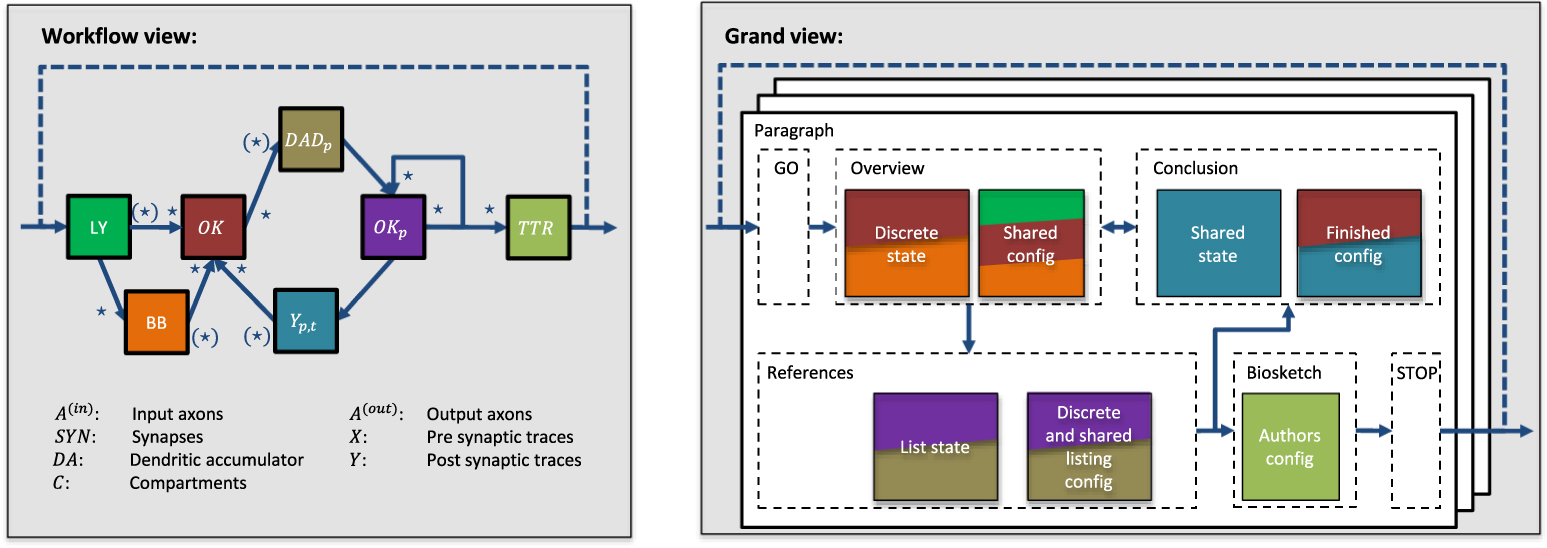
\includegraphics[width=26pc]{./latex-imagenes/fig2.jpg}}
\caption{Nota que ``Figura'' está escrito. Hay un punto después del número de la figura, seguido de un espacio. Es una buena práctica explicar brevemente el significado de la figura en la descripción de esta.}\vspace*{-5pt}
\label{fig:uno}
\end{figure*}

\subsection{Figuras}
Cómo se puede apreciar las imágenes pueden ocupar como ancho ambas columnas como en la Figura~\ref{fig:uno} o solo una columna como  en la Figura~\ref{fig:dos}.

\begin{figure}
\centerline{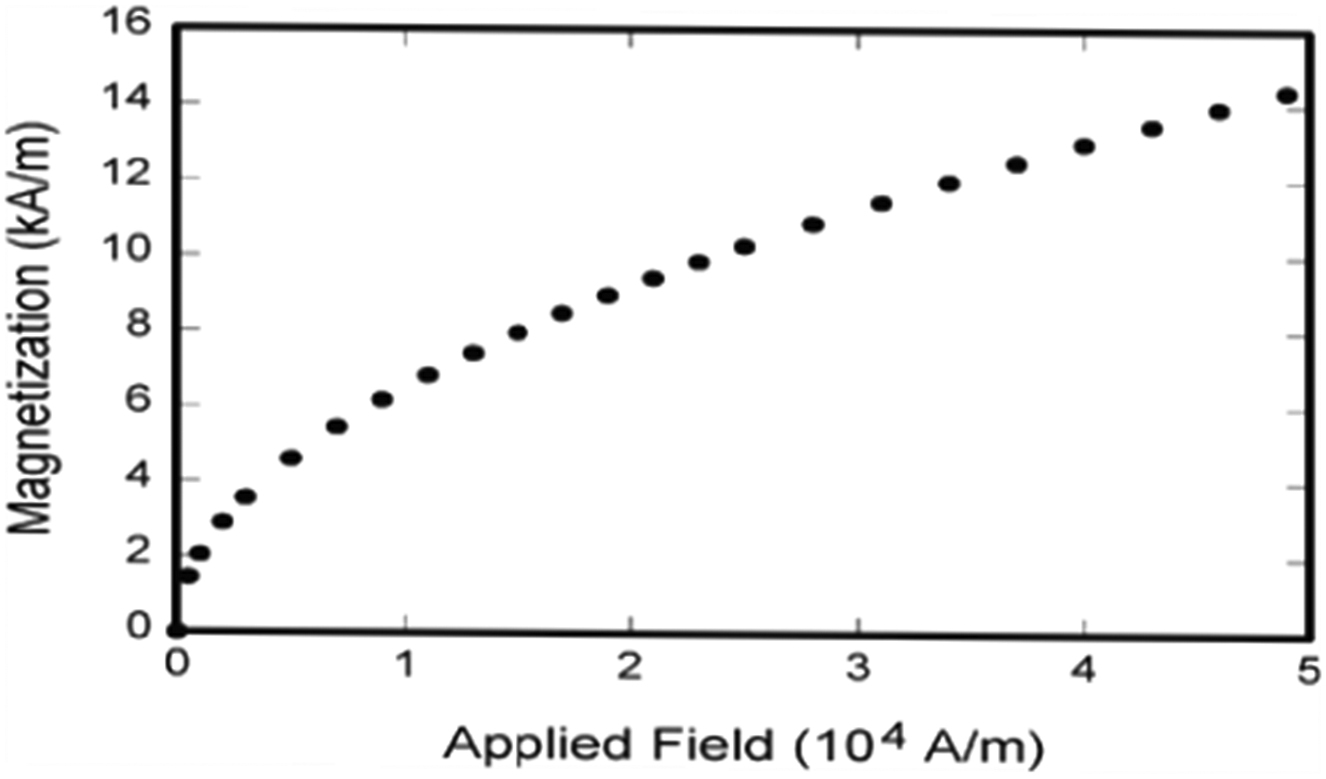
\includegraphics[width=18.5pc]{./latex-imagenes/fig1.jpg}}
\caption{Nota que ``Figura'' está escrito. Hay un punto después del número de la figura, seguido de un espacio. Es una buena práctica explicar brevemente el significado de la figura en la descripción de esta.}
\vspace*{-5pt}
\label{fig:dos}
\end{figure}


\subsection{Tablas}
A continuación se muestra el ejemplo de la inserción de una tabla.


\begin{table}[h]
\vspace*{4pt}
\caption{Unidades para propiedades magneticas.}
\label{table}
\tablefont
\begin{tabular*}{17.5pc}{@{}p{29pt}p{63pt}<{\raggedright}p{80pt}<{\raggedright}@{}}
\toprule
Symbol& 
Quantity& 
Conversión de Gaussian y  CGS EMU a SI$^{\mathrm{a}}$ \\
\colrule
$\Phi $& 
Magnetic flux& 
1 Mx $\to  10^{-8}$ Wb $= 10^{-8}$ V $\cdot$ s \\[3pt]
$B$& 
Magnetic flux density,   magnetic induction& 
1 G $\to  10^{-4}$ T $= 10^{-4}$ Wb/m$^{2}$ \\[3pt]
$H$& 
Magnetic field strength& 
1 Oe $\to  10^{-3}/(4\pi )$ A/m \\[3pt]
$m$& 
Magnetic moment& 
1 erg/G $=$ 1 emu   $\to 10^{-3}$ A $\cdot$ m$^{2} = 10^{-3}$ J/T \\[3pt]
$M$& 
Magnetization& 
1 erg/(G $\cdot$ cm$^{3}) =$ 1 emu/cm$^{3}$   $\to 10^{-3}$ A/m \\[3pt]
4$\pi M$& 
Magnetization& 
1 G $\to  10^{-3}/(4\pi )$ A/m \\
\botrule
\multicolumn{3}{@{}p{17.5pc}@{}}{$^{{\rm a}}$La unidades Gaussian son las mismas como en  CGS EMU para magnetostática; Mx 
$=$ maxwell, G $=$ gauss, Oe $=$ oersted; Wb $=$ weber, V $=$ volt, s $=$ 
second, T $=$ tesla, m $=$ meter, A $=$ ampere, J $=$ joule, kg $=$ 
kilogram, H $=$ henry.}
\end{tabular*}\vspace*{-5pt}
\label{tab1}
\end{table}



\section{ECUACIONES}
Las referencias a las ecuaciones deben mostrarse con un número entre paréntesis. Por ejemplo la ecuación de la recta es

\begin{equation}
y = mx + b.
\label{eq:recta}
\end{equation}

El numero es importante para posteriormente hacer referencia a esa ecuación en la redacción utilizando el numero. Por ejemplo, en~(\ref{eq:recta}) $m$ es la pendiente mientras $b$ es el intercepto.



Si se va a mostrar un desarrollo se debe usar \textit{align}, por ejemplo a continuación se sustituye $x = 2$ en la función $f(x)$, por lo que tenemos 
\begin{align*}
    f(x) &= x^{2} + 3x - 2\\
    f(x=2) &= 2^{2} + 3 \cdot 2 - 2\\
    f(x=2) &= 4 + 6 - 2\\
    f(x=2) &=8.
\end{align*}


\section{LISTS}

Si se utiliza una lista mantenerla lo mas corta que sea posible:

\begin{itemize}
\item[{\ieeeguilsinglright}] {\it Estilo para listas con viñetas}---Este es el estilo que se debe utilizar para las listas con viñetas.
	
\item[{\ieeeguilsinglright}] {\it Puntuación en listas}---Cada elemento de la lista debe finalizar con un punto.

\item[{\ieeeguilsinglright}] {\it Estilo de listas ordenadas}---Usa 1), 2), 3) seguido de  a), b), c), y entonces i), ii), iii); en este orden para crear listas ordenadas anidadas.
\end{itemize}
%\vspace*{3pt}


\section{USO DE REFERENCIAS}
Las referencias deben citarse en el texto. Aparecen como números entre corchetes dependiendo del orden en el que aparezcan en la redacción. Se deben capturar dentro de la  sección Referencias en el orden en que aparecen en el texto. Por ejemplo ``El estudio en \cite{AA1}  muestra que cuando $\ldots$''.




\section{CONCLUSION}
El manuscrito debe incluir direcciones futuras de la investigación. Se recomienda encarecidamente a los autores que no hagan referencia a varias figuras o tablas en la conclusión; estos deben mencionarse en el cuerpo del artículo.
\vspace*{-8pt}


\section{AGRADECIMIENTOS}
Esta sección es opcional. Si los autores creen necesario agradecer a alguien por haber aportado al desarrollo de su proyecto integrador de alguna u otra forma, esta sección esta destinada para esto.


\def\refname{REFERENCES}

\begin{thebibliography}{1}

\bibitem{AA1}
G. M. Amdahl, G. A. Blaauw, and F. P. Brooks, ``Architecture of the IBM System/360,'' {\it IBM J. Res. Dev}., vol. 8, no. 2, pp. 87--101, 1964. (Journal)

\bibitem{BB1}
IBM Corporation, IBM Knowledge Center - IBM Secure Service Container (Secure Service Container). [Online]. Available: {https://www.ibm.com/support/\break knowledgecenter/en/HW11R/com.ibm.hwmca.kc\_se.doc/\break introductiontotheconsole/wn2131zaci.html} (URL)

\bibitem{CC1}
J. Williams, ``Narrow-band analyzer,'' Ph.D. dissertation, Dept.  Elect. Eng., Harvard Univ., Cambridge, MA, USA, 1993. (Thesis or dissertation)

\bibitem{DD1}
J. M. P\'erez, R. Berlanga, M. J. Aramburu, and T. B. Pedersen, ``Integrating data warehouses with web data: A survey,'' {\it IEEE Trans. Knowl. Data Eng}., early access, Dec. 21, 2007, doi:10.1109/TKDE.2007.190746. (Preprint)

\bibitem{EE1}
W.-K. Chen, {\it Linear Networks and Systems}. Belmont, CA, USA: Wadsworth,  1993, pp. 123--135. (Book)

\bibitem{FF1}
S. P. Bingulac, ``On the compatibility of adaptive controllers,'' in {\it Proc. 4th Ann. Allerton Conf. Circuits Syst. Theory}, 1994,  pp. 8--16. (Conference proceedings)

\bibitem{GG1}
K. Elissa, ``An overview of decision theory,'' unpublished. (Unpublished manuscript)

\bibitem{HH1}
R. Nicole, ``The last word on decision theory,'' {\it J. Comput. Vis.}, submitted for publication. (Pending publication)

\bibitem{II1}
C. J. Smith and J. S. Smith, Rocky Mountain Research Laboratories, Boulder, CO, USA, private communication, 1992. (Private communication)
\end{thebibliography}\vspace*{-8pt}


\begin{IEEEbiography}{Cuadros Romero Francisco Javier}{\,}Todas las biografías se limitan a un párrafo y deben ser muy sintéticas. Se puede agregar la carrera en la cual el estudiante esta enrolado. Se pueden mencionar los 3 intereses principales del estudiante. Asi como su aspiración en el corto y mediano plazo. Al final de la biografia de cada estudiante se debe agregar el enlace a su pagina personal en Github: 
%\vadjust{\vfill\pagebreak}
\end{IEEEbiography}

\begin{IEEEbiography}{Neri Pérez Giovany Humberto}{\,}es un estudiante de la ingeniería en Tecnologías de la Información y Comunicaciones con una pasión desbordante por los videojuegos, el anime y los ``corridos tumbados''. Nacido y criado en  Tetepango, desde temprana edad mostró un gran interés por la tecnología y los avances en el campo de la informática. Aunque sus intereses pueden parecer diversos, Giovany encuentra inspiración en la creatividad y la narrativa tanto de los videojuegos como del anime. Estos medios le han enseñado la importancia de la perseverancia, la resolución de problemas y el trabajo en equipo. El objetivo principal de Giovany es completar sus estudios universitarios en ITICs, con especialización en ciberseguridad. Sueña con trabajar en el campo de la ciberseguridad, protegiendo sistemas e información vital de ataques cibernéticos y contribuyendo así a la seguridad digital de las organizaciones.
\end{IEEEbiography}

\end{document}

